%\documentstyle[10pt,twoside]{article}
%\documentstyle[twoside]{article}
\documentclass[twoside]{article}
\setlength{\oddsidemargin}{0.25 in}
\setlength{\evensidemargin}{-0.25 in}
\setlength{\topmargin}{-0.6 in}
\setlength{\textwidth}{6.5 in}
\setlength{\textheight}{8.5 in}
\setlength{\headsep}{0.75 in}
\setlength{\parindent}{0 in}
\setlength{\parskip}{0.1 in}

\usepackage{graphicx}
\usepackage{url}
\usepackage{bm}
\usepackage{amsmath}
\usepackage{verbatim}
\usepackage{float}
%
% The following commands sets up the lecnum (lecture number)
% counter and make various numbering schemes work relative
% to the lecture number.
%
\newcounter{lecnum}
\renewcommand{\thepage}{\thelecnum-\arabic{page}}
\renewcommand{\thesection}{\thelecnum.\arabic{section}}
\renewcommand{\theequation}{\thelecnum.\arabic{equation}}
\renewcommand{\thefigure}{\thelecnum.\arabic{figure}}
\renewcommand{\thetable}{\thelecnum.\arabic{table}}
\newcommand{\dnl}{\mbox{}\par}

%
% The following macro is used to generate the header.
%
\newcommand{\lecture}[4]{
   \pagestyle{myheadings}
   \thispagestyle{plain}
   \newpage
   \setcounter{lecnum}{#1}
   \setcounter{page}{1}
   \noindent
   \begin{center}
   \framebox{
      \vbox{\vspace{2mm}
    \hbox to 6.28in { {\bf CMPSCI~677~~~Operating Systems
                        \hfill Spring 2017} }
       \vspace{4mm}
       \hbox to 6.28in { {\Large \hfill Lecture #1: #2  \hfill} }
       \vspace{2mm}
       \hbox to 6.28in { {\it Lecturer: #3 \hfill Scribe: #4} }
      \vspace{2mm}}
   }
   \end{center}
   \markboth{Lecture #1: #2}{Lecture #1: #2}
   \vspace*{4mm}
}

%
% Convention for citations is authors' initials followed by the year.
% For example, to cite a paper by Leighton and Maggs you would type
% \cite{LM89}, and to cite a paper by Strassen you would type \cite{S69}.
% (To avoid bibliography problems, for now we redefine the \cite command.)
%
\renewcommand{\cite}[1]{[#1]}

% \input{epsf}

%Use this command for a figure; it puts a figure in wherever you want it.
%usage: \fig{NUMBER}{FIGURE-SIZE}{CAPTION}{FILENAME}
\newcommand{\fig}[4]{
            %\vspace{0.2 in}
            \centerline{\includegraphics[scale=#2]{#4}}
            \begin{center}
            Figure \thelecnum.#1:~#3
            \end{center}
    }

% Use these for theorems, lemmas, proofs, etc.
\newtheorem{theorem}{Theorem}[lecnum]
\newtheorem{lemma}[theorem]{Lemma}
\newtheorem{proposition}[theorem]{Proposition}
\newtheorem{claim}[theorem]{Claim}
\newtheorem{corollary}[theorem]{Corollary}
\newtheorem{definition}[theorem]{Definition}
\newenvironment{proof}{{\bf Proof:}}{\hfill\rule{2mm}{2mm}}

% Some useful equation alignment commands, borrowed from TeX
\makeatletter
\def\eqalign#1{\,\vcenter{\openup\jot\m@th
  \ialign{\strut\hfil$\displaystyle{##}$&$\displaystyle{{}##}$\hfil
      \crcr#1\crcr}}\,}
\def\eqalignno#1{\displ@y \tabskip\@centering
  \halign to\displaywidth{\hfil$\displaystyle{##}$\tabskip\z@skip
    &$\displaystyle{{}##}$\hfil\tabskip\@centering
    &\llap{$##$}\tabskip\z@skip\crcr
    #1\crcr}}
\def\leqalignno#1{\displ@y \tabskip\@centering
  \halign to\displaywidth{\hfil$\displaystyle{##}$\tabskip\z@skip
    &$\displaystyle{{}##}$\hfil\tabskip\@centering
    &\kern-\displaywidth\rlap{$##$}\tabskip\displaywidth\crcr
    #1\crcr}}
\makeatother

% **** IF YOU WANT TO DEFINE ADDITIONAL MACROS FOR YOURSELF, PUT THEM HERE:



% Some general latex examples and examples making use of the
% macros follow.

\begin{document}

%FILL IN THE RIGHT INFO.
%\lecture{**LECTURE-NUMBER**}{**DATE**}{**LECTURER**}{**SCRIBE**}
\lecture{24}{April 25}{Prashant Shenoy}{\textbf{Abhishek Somani}}

\section{Big Data Application}
Nowadays, large volumes of data (Terabytes and Petabytes) are being collected and analyzed at unprecedented scales. The abundance of data and the need for collecting, storing, and processing them have raised many technical challenges for the Big Data applications. Parallel and distributed computing is a matter of paramount importance especially for mitigating scale and timeliness challenges. 

Below are the various big data distributed computing platforms:

\section{Map Reduce Model}
MapReduce is a framework for processing parallelizable problems across large datasets using a large number of computers (nodes), collectively referred to as a cluster (if all nodes are on the same local network and use similar hardware) or a grid (if the nodes are shared across geographically and administratively distributed systems, and use more heterogenous hardware). Processing can occur on data stored either in a filesystem (unstructured) or in a database (structured). MapReduce can take advantage of the locality of data, processing it near the place it is stored in order to minimize communication overhead.

Example: Let's say we have huge dataset of number (or may be words in a document) which need to be sorted (or frequency of words). Suppose we have multiple machines. Then each machine could take a chunk of data and sort it. Later, all these sorted chunks chould be merge together similar to merge sort algorithm. However, this requires huge communication between the machines during merge phase. To overcome this problem, let's say we know the range of numbers. In such a case, we could follow the bucket sort paradigm where each machine sorts a specific range of numbers. This way, inter-machine communication can be reduced. 

\textbf{Question} : What if the numbers are not evenly distributed. Then some machines would get more data to sort compared to other machines ? \\
\textbf{Answer} : This is the disadvantage of the approach. So, it is a design tradeoff. 

\begin{figure}[H]
\centering
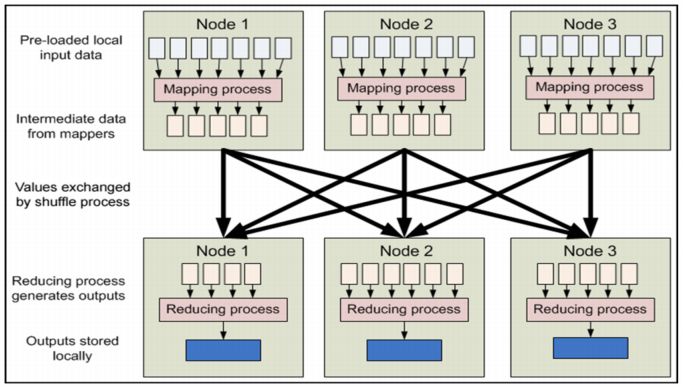
\includegraphics[width=100mm]{map-reduce.png}
\caption{Map Reduce example\label{overflow}}
\end{figure}

\begin{description}
  \item[Map Step] : Each worker node applies the "map()" function to the local data, and writes the output to a temporary storage. A master node ensures that only one copy of redundant input data is processed.
  \item[Shuffle Step] :  Worker nodes redistribute data based on the output keys (produced by the "map()" function), such that all data belonging to one key is located on the same worker node.
  \item[Reduce Step] : Worker nodes now process each group of output data, per key, in parallel.
\end{description}

Its easy for developing distributed parallel processing since developer needs to write only the Map and Reduce functions.

\textbf{Question} : Reduce processes are on certain nodes. Are the map processes only on certain nodes ? \\
\textbf{Answer} : It is configurable and dynamic. During initial processing, a lot of nodes can be assigned map processes. After Shuffle, the same nodes could also be assigned reduce processes. In general, a node runs a bunch of map and reduce processes. 

\subsection{Other Programming Models}
\begin{description}
\item[Apache Tez] An application framework which allows for a complex directed-acyclic-graph of tasks for processing data. 
\item[Microsoft Naiad]Naiad is system for data-parallel dataflow computation which attempts to raise the levels of abstraction used by programmers from an imperative sequence of MapReduce-style statements, to involve higher level concepts of loops and streaming.
\item[Spark]Apache Spark is a fast and general engine for big data processing, with built-in modules for streaming, SQL, machine learning and graph processing. DAG with in memory resilient data sets.
\item[Flink]Apache Flink® is an open-source stream processing framework for distributed, high-performing, always-available, and accurate data streaming applications. DAG models extended to cyclic graphs.
\end{description}

\section{Hadoop Big Data Platform}Hadoop is an implementation of Map-Reduce framework. It is an open-source software framework for storing data and running applications on clusters of commodity hardware. It provides massive storage for any kind of data, enormous processing power and the ability to handle virtually limitless concurrent tasks or jobs. It has :
\begin{itemize}
\item \textbf{store managers} : HDFS, HBASE, Kafka, etc (replication for fault tolerence.
\item \textbf{processing framework} : Map-reduce, Spark, etc
\item \textbf{resource managers} : Some of the concepts of distributed scheduling are also adpoted since they need to serve multiple users. Example : Yarm, Mesos, etc
\end{itemize}

\section{Ecosystem Overview}
Based on the requirements different types of frameworks can be used. For example, if user wants to process the data that have lot of graphs then Graph processing framework Giraph can be used. There are machine learning frameworks like MLLib, Oyyx, Tensorflow that are also designed to run to on Hadoop. If a user wants to input data to these distributed processing framework, he could use applications like hive to easily write map-reduce codes. For real time data processing where data is generated continuously by some external source, framework like Spark Storm etc could be used.
\begin{figure}[H]
\centering
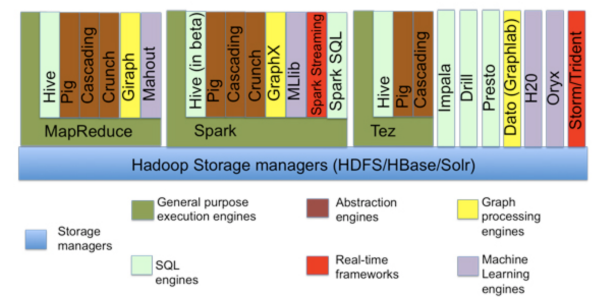
\includegraphics[width=150mm]{Ecosystem.png}
\caption{Ecosystem overview \label{overflow}}
\end{figure}

\subsection{Spark Platform}
Apache Spark is a powerful open source processing engine built around speed, ease of use, and sophisticated analytics. It was originally developed at UC Berkeley in 2009.
\begin{figure}[H]
\centering
%\includegraphics[width=100mm]{Spark.png}
\caption{Spark Platform \label{overflow}}
\end{figure}
\begin{description}
\item[Spark SQL]: Spark SQL is a Spark module for structured data processing. It provides a programming abstraction called DataFrames and can also act as distributed SQL query engine. It enables unmodified Hadoop Hive queries to run up to 100x faster on existing deployments and data. It also provides powerful integration with the rest of the Spark ecosystem (e.g., integrating SQL query processing with machine learning).
\item[Spark Streaming]Many applications need the ability to process and analyze not only batch data, but also streams of new data in real-time. Running on top of Spark, Spark Streaming enables powerful interactive and analytical applications across both streaming and historical data, while inheriting Spark’s ease of use and fault tolerance characteristics. It readily integrates with a wide variety of popular data sources, including HDFS, Flume, Kafka, and Twitter.
\item[MLlib]Built on top of Spark, MLlib is a scalable machine learning library that delivers both high-quality algorithms (e.g., multiple iterations to increase accuracy) and blazing speed (up to 100x faster than MapReduce). The library is usable in Java, Scala, and Python as part of Spark applications, so that you can include it in complete workflows.
\item[GraphX]GraphX is a graph computation engine built on top of Spark that enables users to interactively build, transform and reason about graph structured data at scale. It comes complete with a library of common algorithms.
\end{description}
\textbf{Adavatages of Spark}
\begin{itemize}
\item \textbf{Speed :} Run programs up to 100x faster than Hadoop MapReduce in memory, or 10x faster on disk.Apache Spark has an advanced DAG execution engine that supports acyclic data flow and in-memory computing.
\item \textbf{Ease of Use:} Spark offers over 80 high-level operators that make it easy to build parallel apps. And you can use it interactively from the Scala, Python and R shells.
\item \textbf{Generality :} Combine SQL, streaming, and complex analytics.Spark powers a stack of libraries including SQL and DataFrames, MLlib for machine learning, GraphX, and Spark Streaming. You can combine these libraries seamlessly in the same application.
\item \textbf{Runs Everywhere:} Spark runs on Hadoop, Mesos, standalone, or in the cloud. It can access diverse data sources including HDFS, Cassandra, HBase, and S3.
\end{itemize}

\subsection{Resilient Distributed Datasets (RDDs)}
The Resilient Distributed Dataset is a concept at the heart of Spark. It is designed to support in-memory data storage, distributed across a cluster in a manner that is demonstrably both fault-tolerant and efficient. Fault-tolerance is achieved, in part, by tracking the lineage of transformations applied to coarse-grained sets of data. Efficiency is achieved through parallelization of processing across multiple nodes in the cluster, and minimization of data replication between those nodes. Once data is loaded into an RDD, two basic types of operation can be carried out:
\begin{description}
\item[Transformations] create a new RDD by changing the original through processes such as mapping, filtering, and more;
\item[Actions,] such as counts, which measure but do not change the original data.
The original RDD remains unchanged throughout. The chain of transformations from RDD1 to RDDn are logged, and can be repeated in the event of data loss or the failure of a cluster node.
\end{description}
Where possible, these RDDs remain in memory, greatly increasing the performance of the cluster, particularly in use cases with a requirement for iterative queries or processes.

\begin{figure}[H]
\centering
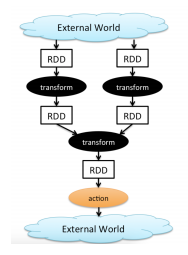
\includegraphics[width=50mm]{RDD.png}
\caption{RDD \label{overflow}}
\end{figure}

\textbf{Question} : Does Spark do exact as Map-reduce except for caching? \\
\textbf{Answer} : Spark has potential to do more than that. Map-reduce can be implemented the same way.

\section{Distributed system Security}
The introduction of distributed systems and the use of networks for carrying data between computers is a major factor that has affected security. Security is a complicated business that wasn't given much thought until uses of computer networks increased and the potential for abuse became interesting 
\subsection{Authentication}
In simple terms, authentication is identification plus verification. Identification is the procedure whereby an entity claims a certain identity, while verification is the procedure whereby that claim is checked. Thus the correctness of an authentication relies heavily on the verification procedure employed.
The entities in a distributed system that can be distinctly identified are collectively referred to as principals.
There are three main types of authentication of interest in a distributed system:
(A1) message content authentication — verifying that the content of a message received is the same as
when it was sent;
(A2) message origin authentication — verifying that the sender of a received message is the same one
recorded in the sender field of the message; and
(A3) general identity authentication — verifying that the a principal’s identity is as claimed.
\subsubsection{Authentication Protocols}
\begin{description}

\item[ Authentication Protocol ap1.0]Perhaps the simplest authentication protocol we can imagine is one where Alice simply sends a message to Bob saying she is Alice. The flaw here is obvious - there is no way for Bob actually to know that the person sending the message “I am Alice” is indeed Alice. For example,Trudy (the intruder) could just as well send such a message.

\item[Authentication Protocol ap2.0] If Alice has a well-known network address (e.g., an IP address) from which she always communicates, Bob could attempt to authenticate Alice by verifying that the source address on the IP datagram carrying the authentication message matches Alice’s well-known address. In this case, Alice would be authenticated. IP spoofing can easily fail this protocol.

\item[ Authentication Protocol ap3.0] One classic approach to authentication is to use a secret password. We have PINs to identify ourselves to automatic teller machines and login passwords for operating systems. The password is a shared secret between the authenticator and the person being authenticated. Telnet and FTP use password authentication. The security flaw here is clear. If someone eavesdrops on Alice’s communication, then it can learn Alice’s password. Lest you think this is unlikely, consider the fact that when you Telnet to another machine and log in, the login password is sent unencrypted to the Telnet server. Someone connected
to the Telnet client or server’s LAN can possibly sniff (read and store) all
packets transmitted on the LAN and thus steal the login password. In fact, this is a
well-known approach for stealing passwords 

\item[Authentication Protocol ap3.1] for fixing ap3.0 is naturally idea would be to encrypt the password. By encrypting the password, we can prevent someone from learning Alice’s password. If we assume that Alice and Bob share a symmetric secret key, $K_{A–B}$, then Alice can encrypt the password and send her identification message, “I am Alice,” and her encrypted password to Bob. Bob then decrypts the password and, assuming the password is correct, authenticates Alice. Bob feels comfortable in authenticating Alice since Alice not only knows the password, but also knows the shared secret key value needed to encrypt the password.  The issue here is : the use of cryptography here does not solve the authentication problem. Bob is subject to a replay attack: someone now need only eavesdrop on Alice’s communication, record the encrypted version of the password, and play back the encrypted version of the password to Bob to pretend that she is Alice. 

\item[Authentication Protocol ap4.0]The problem with ap3.1 is that the same password is used over and over again. One way to solve this problem would be to use nonces - one in a life time number. Alice and Bob could agree on a sequence of passwords (or on an algorithm for generating passwords) and use each password only once, in sequence. Ap 4.0 also uses symmetric keys for encryption.

\item[Authentication Protocol ap5.0] A protocol that uses public key cryptograhpy in a manner analogous to the use of symmetric key cryptographty in protocol ap4.0 is protocol ap5.0. Since ap5.0 uses public key techniques, it requires that Bob retrieve Alice's public key. Here, public-key encryption is also known as asymmetric-key encryption. public-key encryption uses two different keys at once -- a combination of a private key and a public key. The private key is known only to your computer, while the public key is given by your computer to any computer that wants to communicate securely with it. To decode an encrypted message, a computer must use the public key, provided by the originating computer, and its own private key. 

\end{description}
\end{document}
